\documentclass[11pt]{article}
\usepackage[utf8]{inputenc}
\usepackage[T1]{fontenc}
\usepackage[margin=1in]{geometry}
\usepackage{amsmath,amssymb,bm}
\usepackage{booktabs}
\usepackage{graphicx}
\usepackage{caption}
\usepackage{subcaption}
\usepackage{float}
\usepackage{hyperref}
\usepackage[numbers,sort&compress]{natbib}
\hypersetup{colorlinks=true,linkcolor=blue,citecolor=blue,urlcolor=blue}
\graphicspath{{figures/}}

\title{\textbf{Sparse Counterfactual Attribution of Crop-Yield Anomalies\\to Extreme-Weather Drivers}}
\author{Tran Dai Phong Lam\\FPT University}
\date{}

\begin{document}
\maketitle

\begin{abstract}
Machine-learning studies of crop yield usually optimize average predictive accuracy, but
agricultural risk management often needs a different answer: why did a particular
crop-state-year fall abnormally below its expected yield? We present Sparse
Counterfactual Anomaly Attribution (SCAA), a model-based framework that detects
detrended low-yield anomalies and attributes each event to sparse, physically grouped
extreme-weather drivers. Daily NASA POWER weather and USDA yield records are aggregated
for four crops, twelve U.S. states, and 1990--2025. A forward-time ExtraTrees yield
model reproduces strong predictive skill, with $R^2=0.809$ for 2016--2021 and
$R^2=0.808$ for 2019--2025. After crop-state detrending, 214 of 1,257 observations are
flagged as low-yield anomalies. The main grouped-SCAA attribution method explains
anomalies with heat, drought/dry-spell, frost/cold, excess-rain, and radiation driver
groups. It attains a median recoverable fraction of 0.589, classifies 73.4\% of
anomalies as weather-driven, and matches expected heat/drought/moisture groups in
88.6\% of event-year checks for 2012, 2021, and 2022. Observed-analog counterfactuals
provide a robustness check, and crop-specific vulnerability profiles identify which
drivers lower which crops in the fitted residual model. The results are predictive,
model-internal counterfactual explanations, not causal effects.
\end{abstract}

\noindent\textbf{Keywords:} crop yield; extreme weather; counterfactual explanation; yield anomaly; interpretable machine learning; drought; heat stress.

\section{Introduction}
Extreme weather can produce large agricultural losses, with drought, heat, excess
water, and cold events affecting crop production at regional and global scales
\citep{Lesk2016,Zampieri2017,Vogel2019}. Standard crop-yield machine-learning
workflows demonstrate that weather and climate variables can support accurate yield
forecasting \citep{Paudel2021,Meroni2021,Khaki2019,LengHall2020}, but prediction alone
does not answer the event-level question needed for risk interpretation: which weather
driver does the model identify as the strongest contributor for a specific low-yield
crop-state-year?

This paper reframes yield interpretation as anomaly attribution. We first separate
long-run crop-state yield trend from short-run yield variation, following the logic of
detrended yield residual analysis \citep{Ray2015,Lu2017,Meng2024}. We then detect
low-yield anomalies and ask a counterfactual question: what sparse, feasible change to
the weather features would move the predicted detrended residual back toward a normal
season? Unlike feature-importance methods such as SHAP or LIME
\citep{LundbergLee2017,Ribeiro2016}, this produces a recovery quantity in
t ha$^{-1}$ and a crop-specific event claim.

The contribution is not a new yield predictor. The contribution is a reproducible
event-level attribution workflow that combines detrended yield anomalies, physically
grouped extreme-weather drivers, and feasible sparse counterfactual explanations.
Figure~\ref{fig:workflow} summarizes the pipeline.

\begin{figure}[H]
  \centering
  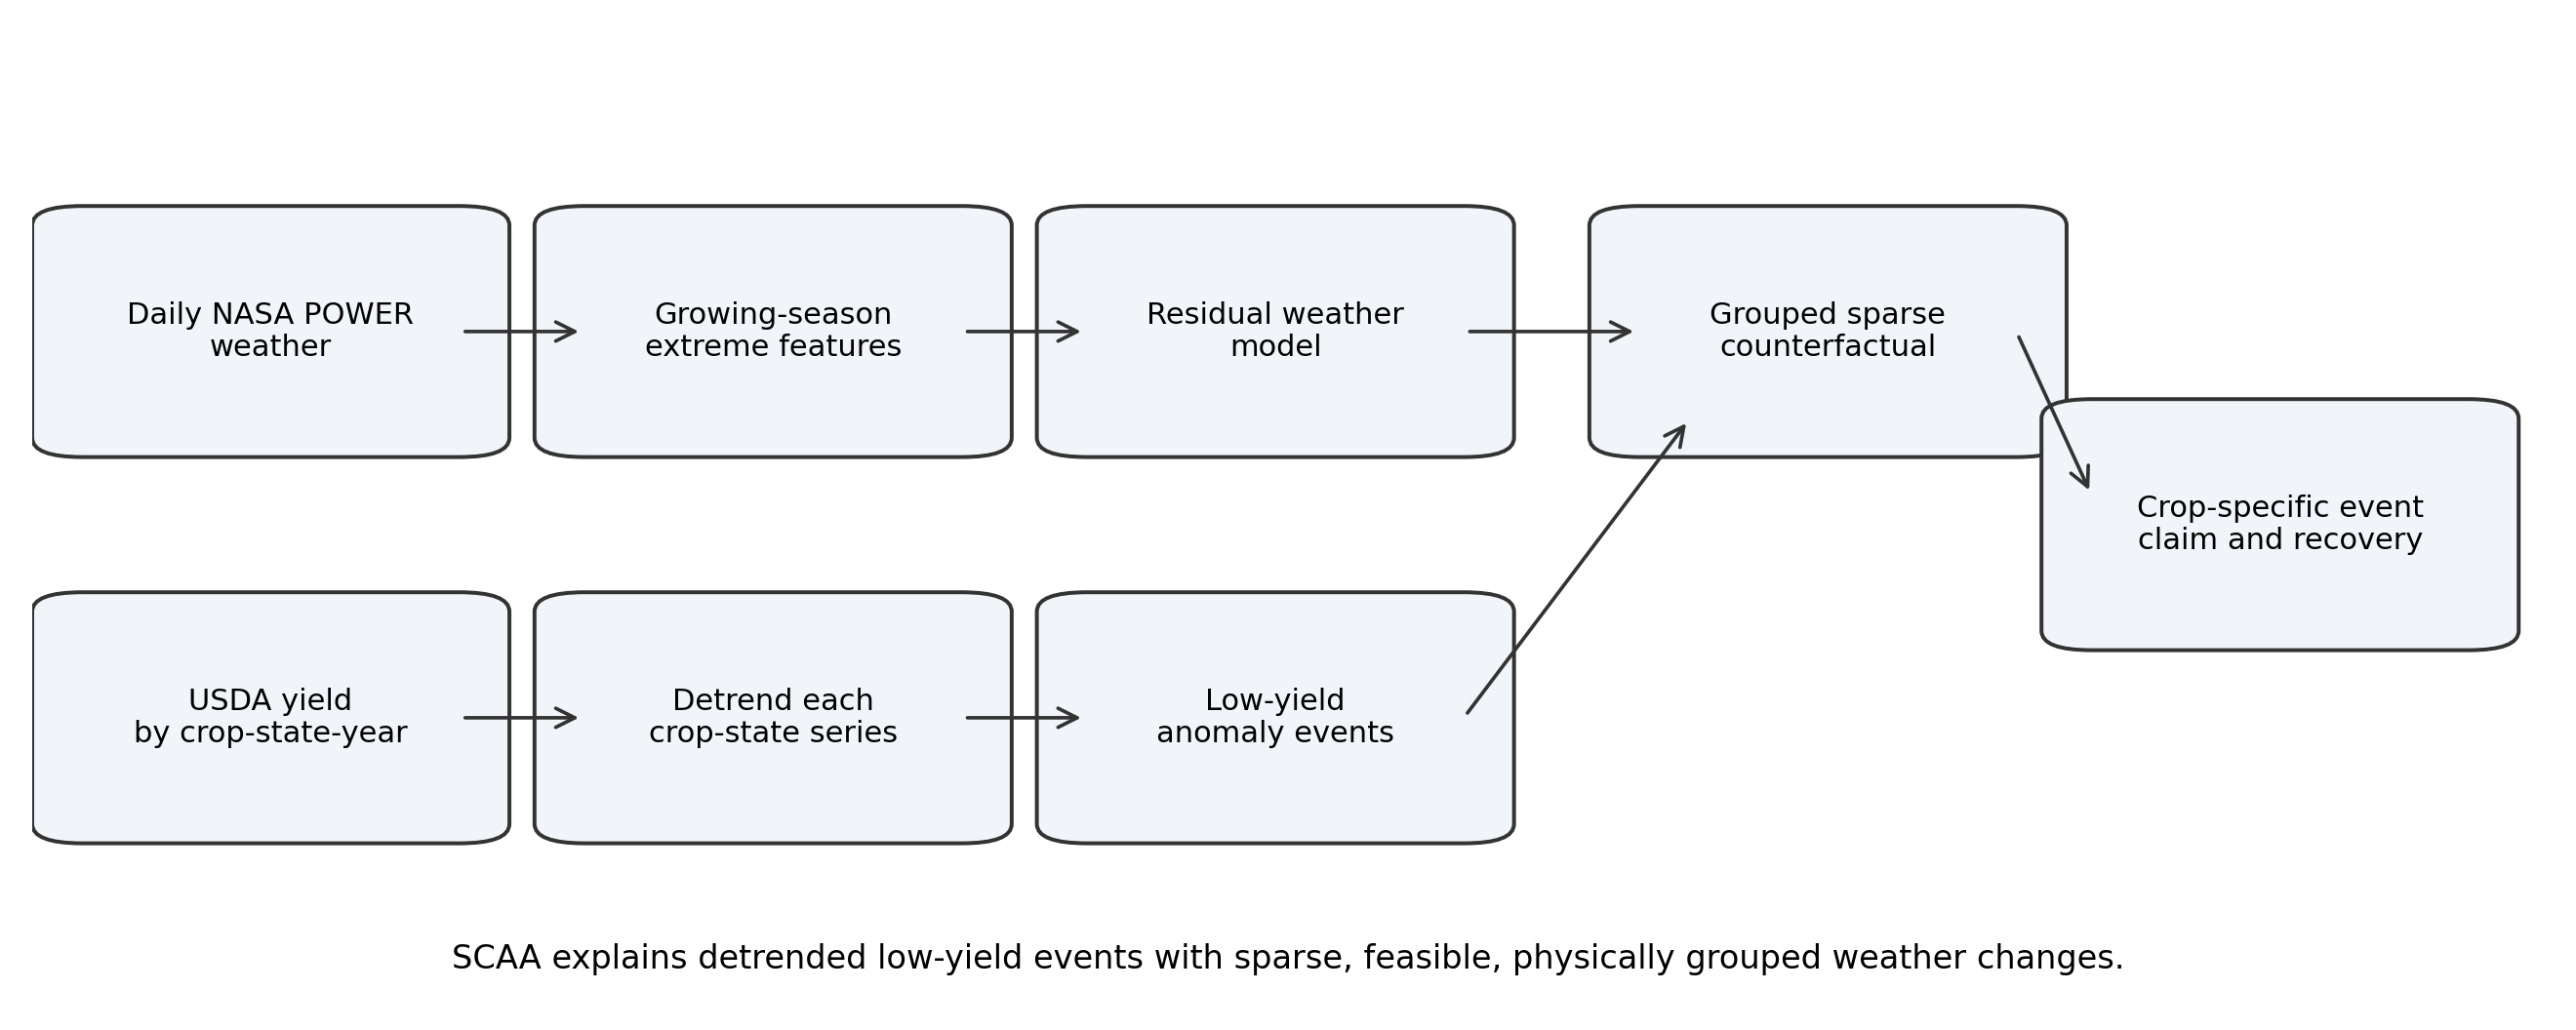
\includegraphics[width=\linewidth]{fig01_method_workflow.png}
  \caption{SCAA workflow. Daily weather and yield records are converted into
  crop-state-year features, detrended anomalies, residual weather models, and grouped
  counterfactual attribution claims.}
  \label{fig:workflow}
\end{figure}

\section{Related Work}
\subsection{Crop-Yield Prediction and Weather Features}
Large-scale crop-yield forecasting has been studied with random forests, neural
networks, and other statistical or machine-learning approaches
\citep{Paudel2021,Khaki2019,Shahhosseini2021}. In-season forecasting under small-data
conditions is also active, especially for grain systems \citep{Meroni2021}. These
studies support the predictive modeling layer of our work, but they mainly optimize
forecasting skill rather than event-level explanation.

\subsection{Extreme-Weather Yield Anomalies}
Prior work links yield anomalies to climate extremes, including heatwaves, drought,
water excess, hot-dry compound events, and crop-specific weather relationships
\citep{Zampieri2017,Vogel2019,Heino2023,Sjulgard2023}. Stage-specific weather effects
are also important because temperature, rainfall, frost, and radiation can matter
differently during crop development \citep{Schierhorn2021}. These studies motivate our
driver groups: heat, drought/dry-spell, frost/cold, excess rainfall, and radiation.

\subsection{Counterfactual and Event Attribution}
Counterfactual explanations ask for minimal changes that would alter a model outcome
\citep{Wachter2018}. Diverse and feasible counterfactual methods emphasize proximity,
sparsity, plausibility, and actionable constraints
\citep{Mothilal2020,Ustun2019,Poyiadzi2020,Verma2024}. Climate-event attribution also
uses counterfactual language, but it requires careful event definition, causal
assumptions, and model validation \citep{Hannart2016,Otto2017,Oldenborgh2021}. We use
the counterfactual form for model-based explanation, while explicitly avoiding strong
causal claims.

\section{Data}
The empirical unit is a crop-state-year. The processed frame contains 1,257
observations for Barley, Canola, Oats, and Wheat across twelve U.S. states from
1990--2025. Yields are in t ha$^{-1}$. Weather features are derived from NASA POWER
daily records and include rainfall totals, dry spells, heavy-rain events, heat days,
heatwaves, growing-degree days, frost/cold metrics, and radiation summaries. Growing
season windows are crop- and state-aware, with spring and winter windows represented
in the processed frame.

\begin{table}[H]
\centering
\caption{Dataset summary by crop.}
\label{tab:dataset_summary}
\resizebox{\linewidth}{!}{%
\begin{tabular}{llllll}
\toprule
crop & observations & states & years & windows & anomalies \\
\midrule
Barley & 283 & 10 & 1990-2025 & spring & 52 \\
Canola & 133 & 6 & 1991-2025 & spring & 21 \\
Oats & 416 & 12 & 1990-2025 & spring & 71 \\
Wheat & 425 & 12 & 1990-2025 & spring, winter & 70 \\
\bottomrule
\end{tabular}%
}
\end{table}

\begin{table}[H]
\centering
\caption{Extreme-weather driver groups used by grouped SCAA.}
\label{tab:driver_groups}
\resizebox{\linewidth}{!}{%
\begin{tabular}{lll}
\toprule
driver\_group & description & features \\
\midrule
heat & High-temperature and heatwave exposure & heat\_days\_30, heat\_days\_35, heatwave\_events\_3d\_30, heat\_degree\_days\_30, season\_tmax\_mean \\
drought & Rainfall deficit, dry days, and dry-spell persistence & rain\_sum, rain\_mean, dry\_days\_1mm, max\_dry\_spell\_1mm, dry\_spell\_events\_7d, dry\_spell\_events\_14d, hot\_dry\_days\_30\_1mm \\
frost\_cold & Cold and frost exposure & frost\_days\_0, cold\_days\_5, min\_tmin, frost\_events\_2d, season\_tmin\_mean \\
excess\_rain & Wetness and heavy-rainfall intensity & wet\_days\_1mm, heavy\_rain\_days\_10, heavy\_rain\_days\_20, max\_1day\_rain, max\_3day\_rain, max\_7day\_rain \\
radiation & Seasonal solar-radiation anomaly & radiation\_sum, radiation\_mean \\
\bottomrule
\end{tabular}%
}
\end{table}


Figure~\ref{fig:data_coverage} shows crop coverage and crop-state density.

\begin{figure}[H]
  \centering
  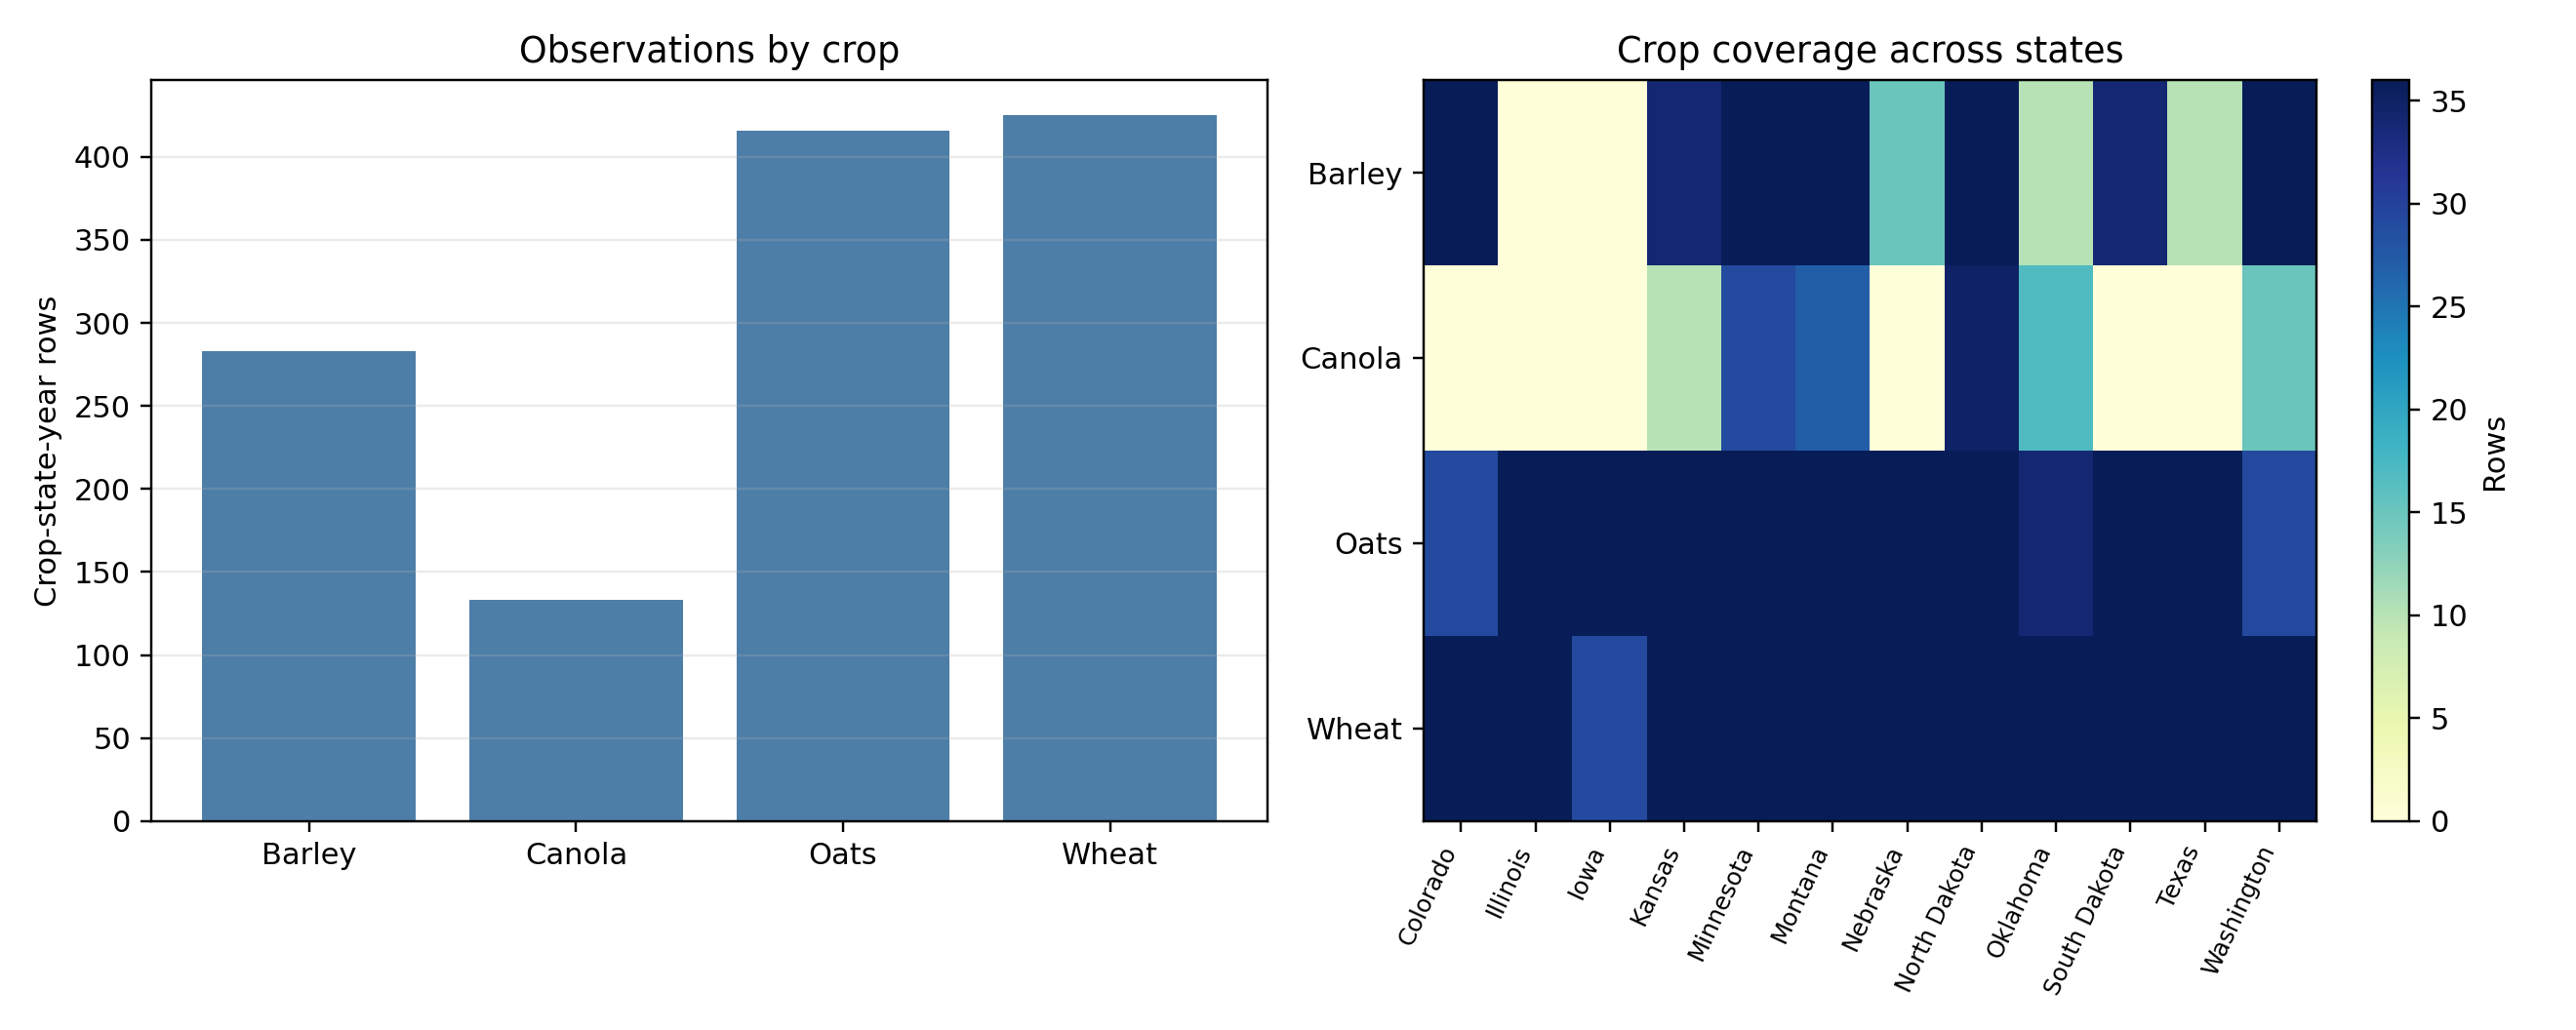
\includegraphics[width=\linewidth]{fig02_data_coverage.png}
  \caption{Data coverage by crop and state.}
  \label{fig:data_coverage}
\end{figure}

\section{Method}
\subsection{Yield Skill Baseline}
We retain a forward-time yield model to verify that the weather and crop-state features
contain predictive signal. Numeric variables are median-imputed and standardized;
categorical crop and state identifiers are one-hot encoded. An ExtraTrees regressor is
trained under two forward-time splits: train through 2015 and test 2016--2021; then
train through 2018 and test 2019--2025.

\subsection{Detrending and Anomaly Detection}
For each crop-state series, a linear trend is fit to yield:
\begin{equation}
  y_{c,s,t} = \alpha_{c,s} + \beta_{c,s} t + \epsilon_{c,s,t}.
\end{equation}
The residual is standardized within each crop-state series. A low-yield anomaly is an
observation with standardized residual below $-1$. This step follows the literature on
separating long-run technology and management trend from weather-sensitive yield
variation \citep{Ray2015,Lu2017,Meng2024}.

\subsection{Grouped Sparse Counterfactual Attribution}
The main paper method is grouped-SCAA. A residual model maps weather and crop-state
features to detrended yield residual. For each low-yield anomaly, grouped-SCAA moves a
single physical driver group toward the observed feasible median for the same
region-window group and evaluates how much of the negative residual is recovered.
For anomaly $i$, the recoverable fraction is:
\begin{equation}
  \phi_i =
  \frac{\min(\hat r_i^{cf} - \hat r_i, \Delta_i)}
       {\Delta_i},
  \quad
  \Delta_i = \max(0, y^{trend}_i - y_i),
\end{equation}
where $\hat r_i$ and $\hat r_i^{cf}$ are the residual-model predictions before and
after the grouped counterfactual edit. A crop-state-year is labelled weather-driven
when $\phi_i \geq 0.5$.

\subsection{Robustness and Extensions}
Observed-analog counterfactuals replace the anomaly weather vector with real normal
seasons from the same crop-state, or the same region-window fallback. This checks
whether high recovery is possible under historically observed weather states.
Crop-specific vulnerability profiles stress-test each crop under adverse observed
driver extremes. An early-warning extension trains anomaly classifiers from early and
early-plus-mid season weather features, with calibration-derived uncertainty bands
\citep{Anderson2024,Singh2024,Farag2025}.

\section{Results}
\subsection{Yield Skill and Anomalies}
The yield model reproduces strong forward-time predictive skill
(Table~\ref{tab:model_performance}; Figure~\ref{fig:yield_prediction}). The 2016--2021
split attains $R^2=0.809$ and RMSE 0.525 t ha$^{-1}$; the 2019--2025 split attains
$R^2=0.808$ and RMSE 0.536 t ha$^{-1}$. After detrending, 214 of 1,257 observations are
flagged as low-yield anomalies. The anomaly timeline peaks in known drought or heat
years, including 2002, 2021, and 2022 (Figure~\ref{fig:anomaly_timeline}).

\begin{table}[!htbp]
\centering
\caption{Forward-time yield performance and anomaly count.}
\label{tab:model_performance}
\resizebox{\linewidth}{!}{%
\begin{tabular}{lllll}
\toprule
evaluation & test\_years & n\_test & r2 & rmse\_t\_ha \\
\midrule
test\_2016\_2021 & 2016-2021 & 209 & 0.809 & 0.525 \\
test\_2019\_2025 & 2019-2025 & 236 & 0.808 & 0.536 \\
window\_spring\_2016\_2021 & 2016-2021 & 164 & 0.842 & 0.475 \\
window\_winter\_2016\_2021 & 2016-2021 & 45 & 0.543 & 0.677 \\
low\_yield\_anomalies & 1990-2025 & 1257 &  & 214 anomalies \\
\bottomrule
\end{tabular}%
}
\end{table}


\begin{figure}[H]
  \centering
  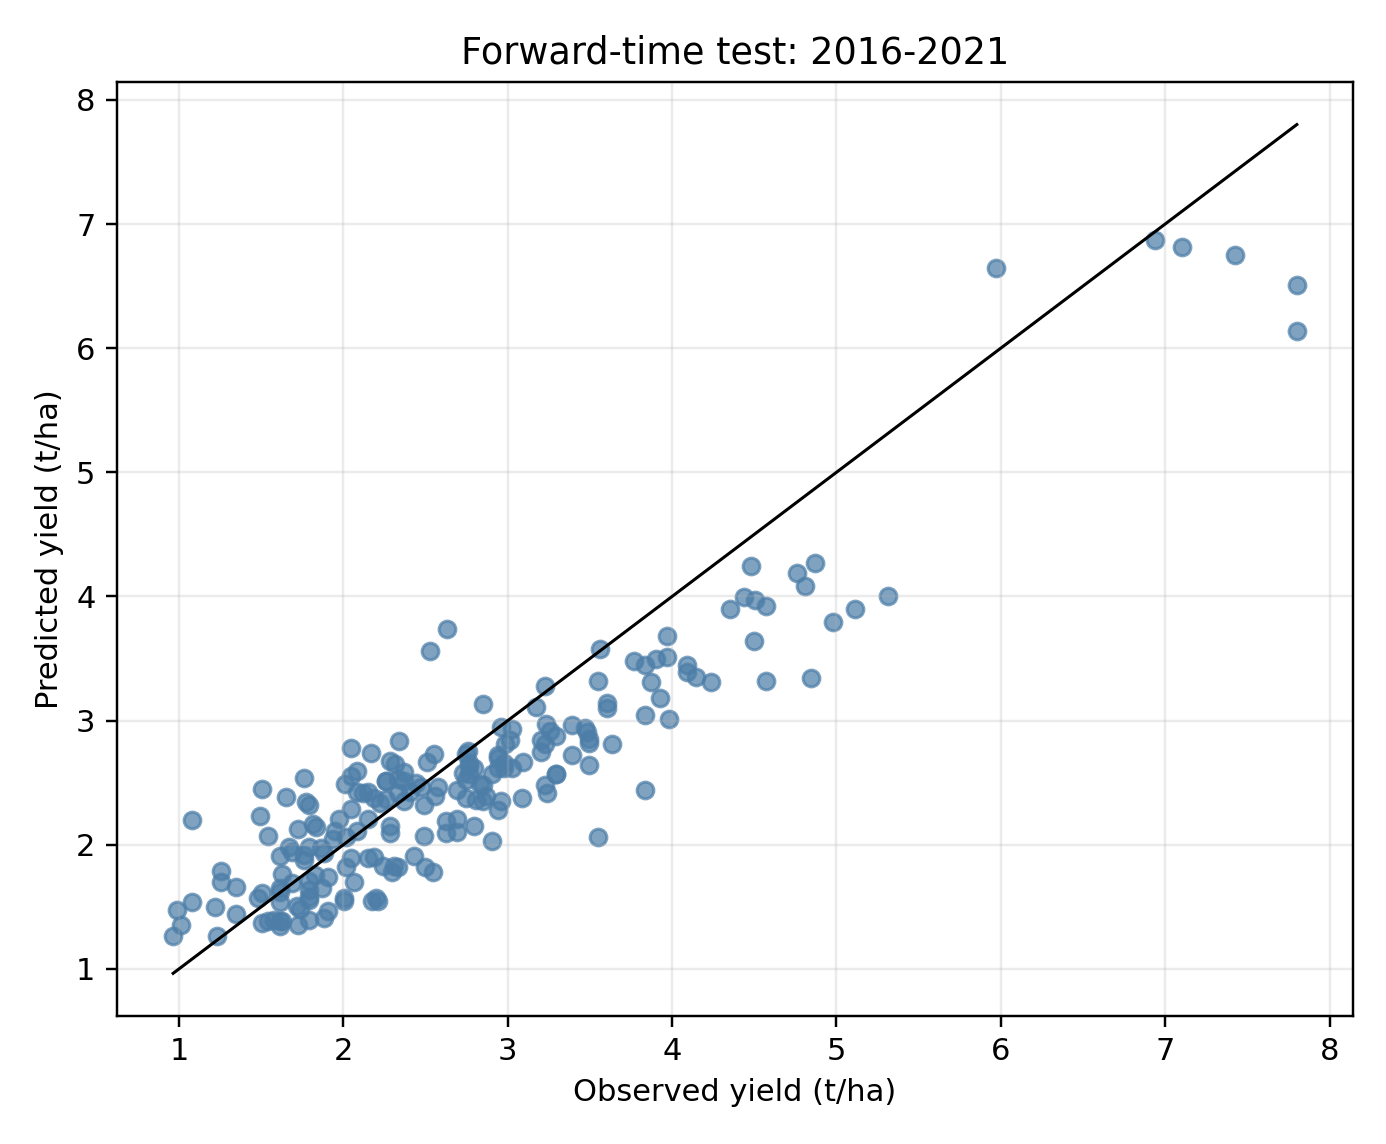
\includegraphics[width=0.68\linewidth]{fig03_yield_prediction.png}
  \caption{Observed versus predicted yield under the forward-time 2016--2021 test.}
  \label{fig:yield_prediction}
\end{figure}

\begin{figure}[H]
  \centering
  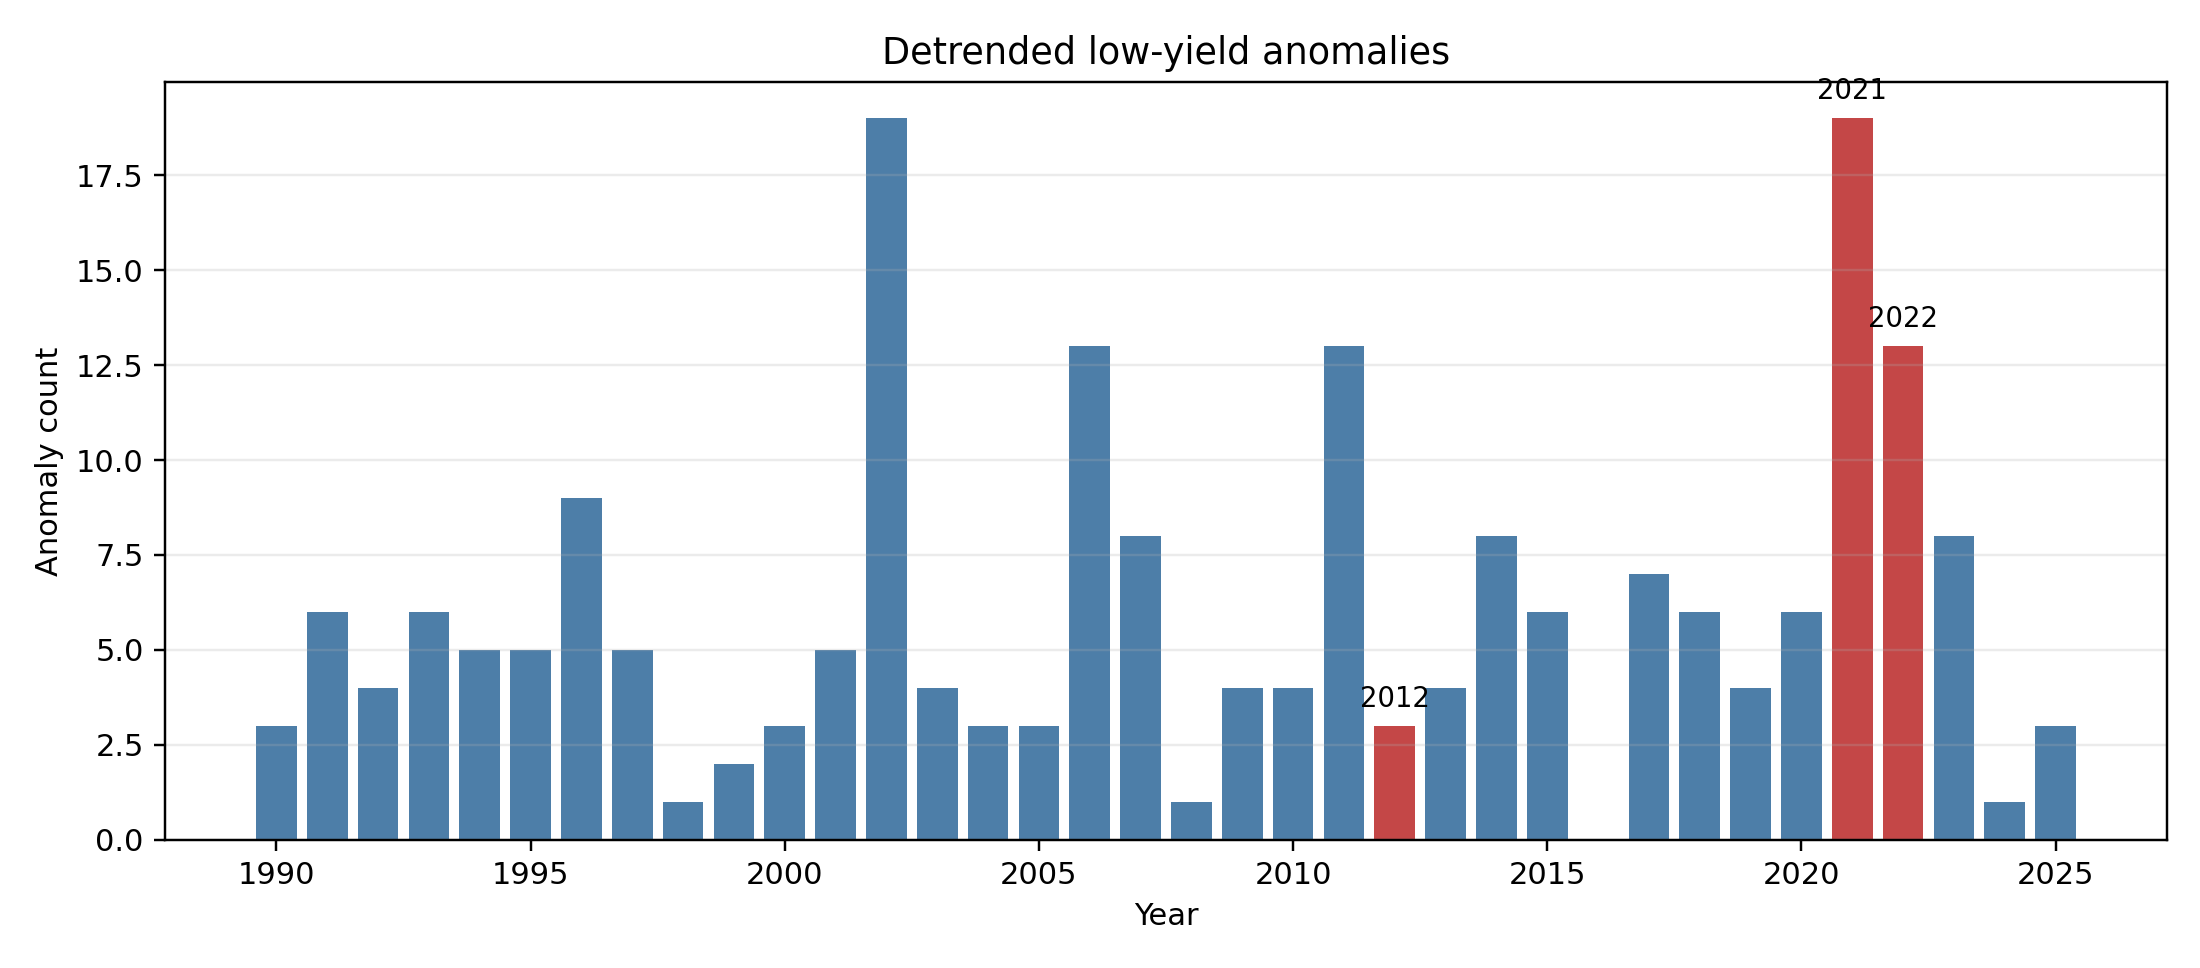
\includegraphics[width=\linewidth]{fig04_anomaly_timeline.png}
  \caption{Low-yield anomaly counts by year, with 2012, 2021, and 2022 highlighted.}
  \label{fig:anomaly_timeline}
\end{figure}

\subsection{Method Comparison}
Table~\ref{tab:method_scorecard} and Figure~\ref{fig:scorecard} compare V1 raw-yield
SCAA, residual-target SCAA, grouped-driver SCAA, observed-analog counterfactuals, crop
vulnerability profiles, and early-warning models. Observed analogs score highest
numerically because they replace the full weather vector with a real normal season; we
therefore use them as robustness evidence rather than the main sparse attribution
method. The main grouped-SCAA method reaches median recoverable fraction 0.589,
weather-driven rate 73.4\%, and event-year expected-driver match 88.6\%.

\begin{table}[H]
\centering
\caption{Method comparison scorecard.}
\label{tab:method_scorecard}
\resizebox{\linewidth}{!}{%
\begin{tabular}{lllll}
\toprule
method & total\_score & median\_recoverable\_fraction & weather\_driven\_rate & event\_expected\_match\_rate \\
\midrule
00\_baseline\_v1\_raw\_yield\_scaa & 6.498 & 0.379 & 0.262 & 0.829 \\
01\_residual\_target\_scaa & 7.511 & 0.482 & 0.472 & 0.629 \\
02\_grouped\_driver\_scaa & 8.745 & 0.589 & 0.734 & 0.886 \\
03\_observed\_analog\_counterfactual & 9.018 & 0.853 & 0.972 & 0.971 \\
04\_crop\_specific\_vulnerability\_profiles & 5.284 &  &  &  \\
05\_early\_mid\_warning\_improved & 4.753 &  &  &  \\
\bottomrule
\end{tabular}%
}
\end{table}


\begin{figure}[H]
  \centering
  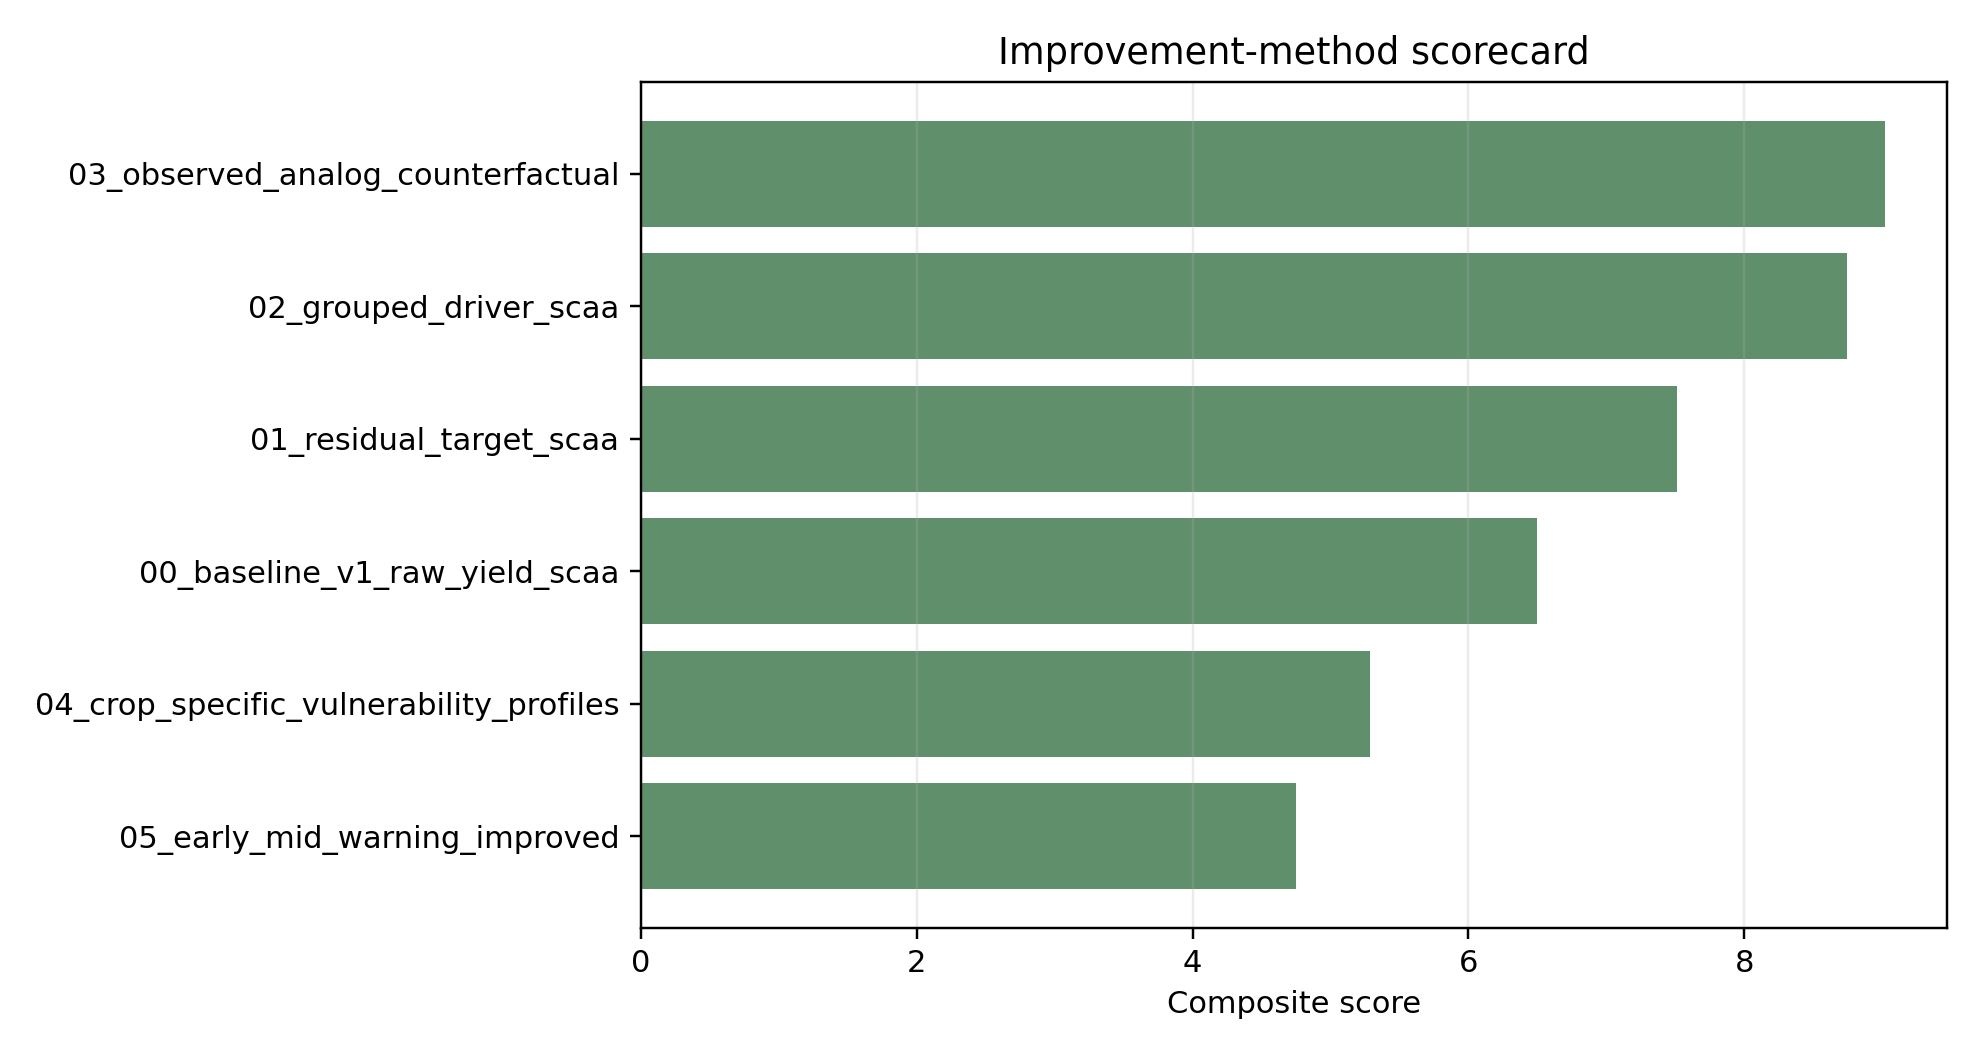
\includegraphics[width=0.86\linewidth]{fig05_method_scorecard.png}
  \caption{Composite scorecard for alternative attribution and warning methods.}
  \label{fig:scorecard}
\end{figure}

\subsection{Grouped Counterfactual Attribution}
Grouped-SCAA produces a recovery fraction and driver group for each anomaly
(Figure~\ref{fig:grouped}). The top crop-specific event claims are shown in
Table~\ref{tab:top_claims}. For example, North Dakota Canola in 2021 is attributed to
drought/dry-spell stress, with a modelled recovery of 0.522 t ha$^{-1}$, while
Minnesota Canola in 2021 is attributed to heat exposure, with a modelled recovery of
0.372 t ha$^{-1}$. These claims are model-based counterfactual recoveries, not direct
causal estimates.

\begin{figure}[H]
  \centering
  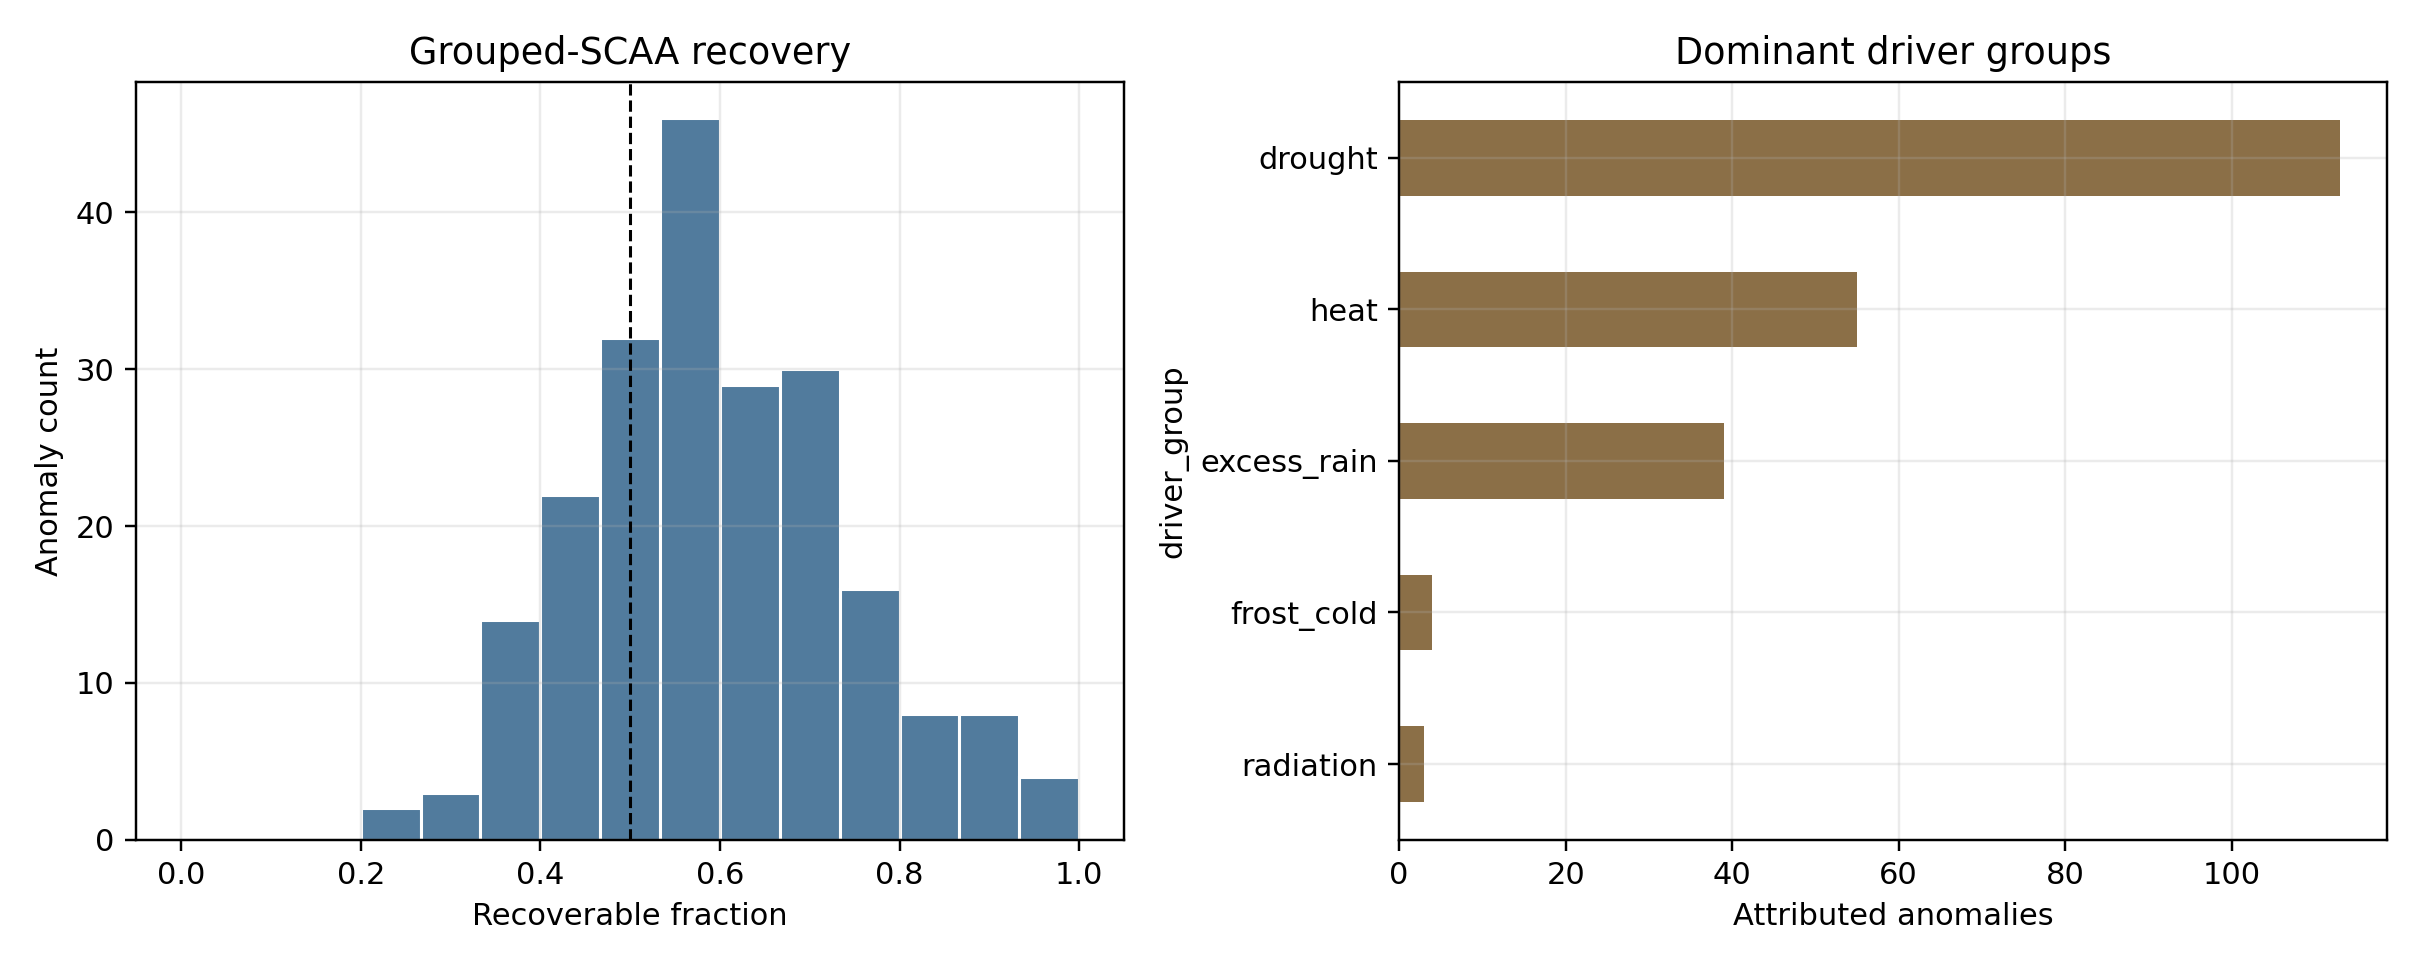
\includegraphics[width=\linewidth]{fig06_grouped_driver_attribution.png}
  \caption{Grouped-SCAA recoverable fraction and dominant driver-group frequency.}
  \label{fig:grouped}
\end{figure}

\begin{table}[H]
\centering
\caption{Top temporal-holdout grouped-SCAA crop-region-year attribution claims.}
\label{tab:top_claims}
\resizebox{\linewidth}{!}{%
\begin{tabular}{llllllll}
\toprule
crop & region & year & driver\_group & dominant\_feature & yield\_gap\_t\_ha & recovered\_gap\_t\_ha & recoverable\_fraction \\
\midrule
Oats & South Dakota & 2006 & drought & rain\_mean & 0.381 & 0.273 & 0.717 \\
Barley & Washington & 2015 & drought & hot\_dry\_days\_30\_1mm & 0.862 & 0.598 & 0.693 \\
Wheat & Washington & 1992 & drought & max\_dry\_spell\_1mm & 0.579 & 0.39 & 0.672 \\
Wheat & Texas & 2009 & drought & dry\_spell\_events\_14d & 0.41 & 0.273 & 0.666 \\
Canola & North Dakota & 2012 & drought & hot\_dry\_days\_30\_1mm & 0.285 & 0.183 & 0.64 \\
\bottomrule
\end{tabular}%
}
\end{table}


\subsection{Event Validation and Robustness}
Event validation focuses on 2012, 2021, and 2022, where heat, drought, and moisture
stress are plausible driver groups from the agronomic and climate-event literature.
Grouped-SCAA matches expected heat/drought/moisture groups in 88.6\% of event-year
attributions, while observed analogs match 97.1\% (Table~\ref{tab:event_validation};
Figure~\ref{fig:event_validation}).

\begin{table}[H]
\centering
\caption{Event validation summary for 2012, 2021, and 2022.}
\label{tab:event_validation}
\resizebox{\linewidth}{!}{%
\begin{tabular}{lllll}
\toprule
method & year & n\_events & expected\_match\_rate & median\_recoverable \\
\midrule
00\_baseline\_v1\_raw\_yield\_scaa & 2012 & 3 & 1.0 & 0.379 \\
00\_baseline\_v1\_raw\_yield\_scaa & 2021 & 19 & 0.842 & 0.27 \\
00\_baseline\_v1\_raw\_yield\_scaa & 2022 & 13 & 0.769 & 0.427 \\
01\_residual\_target\_scaa & 2012 & 3 & 0.667 & 0.465 \\
01\_residual\_target\_scaa & 2021 & 19 & 0.368 & 0.495 \\
01\_residual\_target\_scaa & 2022 & 13 & 1.0 & 0.52 \\
02\_grouped\_driver\_scaa & 2012 & 3 & 1.0 & 0.521 \\
02\_grouped\_driver\_scaa & 2021 & 19 & 0.842 & 0.686 \\
02\_grouped\_driver\_scaa & 2022 & 13 & 0.923 & 0.532 \\
03\_observed\_analog\_counterfactual & 2012 & 3 & 0.667 & 0.584 \\
03\_observed\_analog\_counterfactual & 2021 & 19 & 1.0 & 0.905 \\
03\_observed\_analog\_counterfactual & 2022 & 13 & 1.0 & 0.922 \\
\bottomrule
\end{tabular}%
}
\end{table}


\begin{figure}[H]
  \centering
  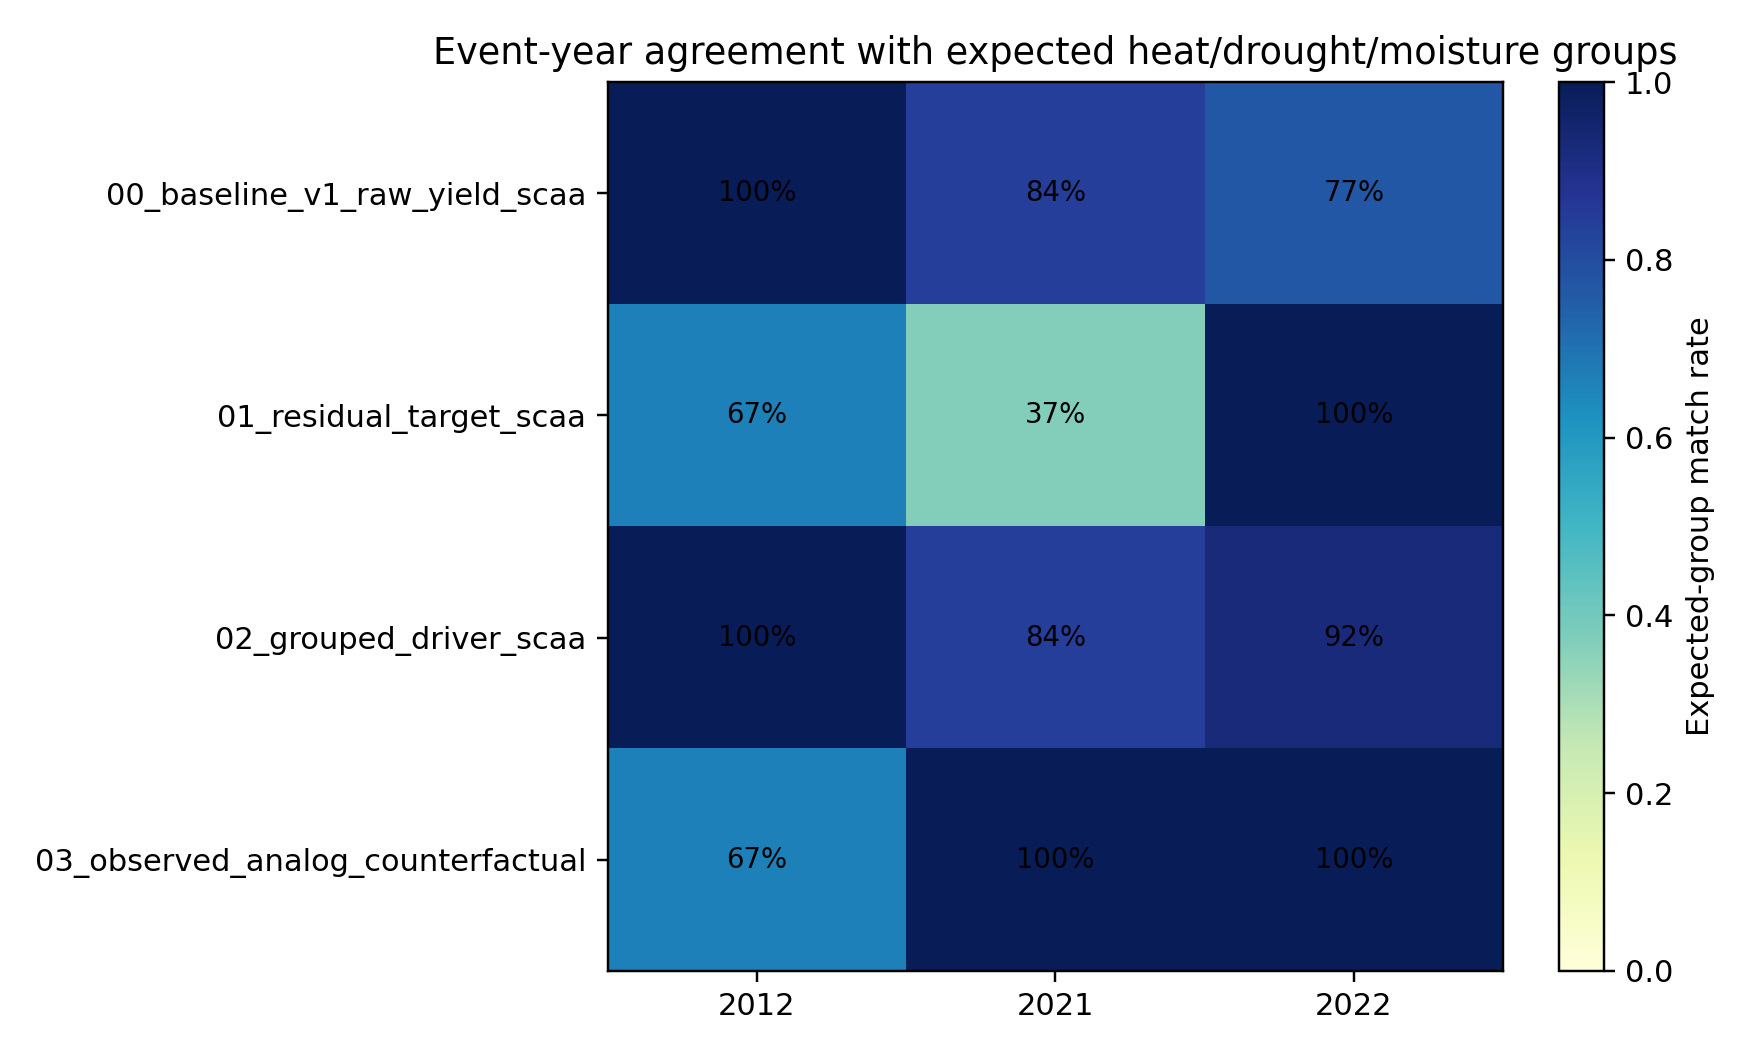
\includegraphics[width=0.82\linewidth]{fig08_event_validation.png}
  \caption{Event-year agreement with expected heat/drought/moisture driver groups.}
  \label{fig:event_validation}
\end{figure}

\subsection{Crop-Specific Vulnerability and Early Warning}
The vulnerability profile answers which weather driver most reduces which crop in the
fitted residual model. Barley is most sensitive to heat exposure, with median residual
effect $-0.134$ t ha$^{-1}$ under adverse observed extremes; Wheat is most sensitive to
drought/dry-spell stress, with median effect $-0.103$ t ha$^{-1}$; and Canola is most
sensitive to heat exposure, with median effect $-0.086$ t ha$^{-1}$.

\begin{table}[!htbp]
\centering
\caption{Top crop-specific yield penalties under adverse observed weather extremes.}
\label{tab:crop_vulnerability}
\resizebox{\linewidth}{!}{%
\begin{tabular}{llll}
\toprule
crop & driver\_group & median\_yield\_penalty\_t\_ha & states\_largest\_penalty \\
\midrule
Barley & heat & 0.134 & Oklahoma (0.253); South Dakota (0.222); Kansas (0.191) \\
Wheat & drought & 0.103 & Washington (0.378); Colorado (0.327); Oklahoma (0.282) \\
Canola & heat & 0.086 & Kansas (0.245); Minnesota (0.167); Oklahoma (0.142) \\
\bottomrule
\end{tabular}%
}
\end{table}


\begin{figure}[H]
  \centering
  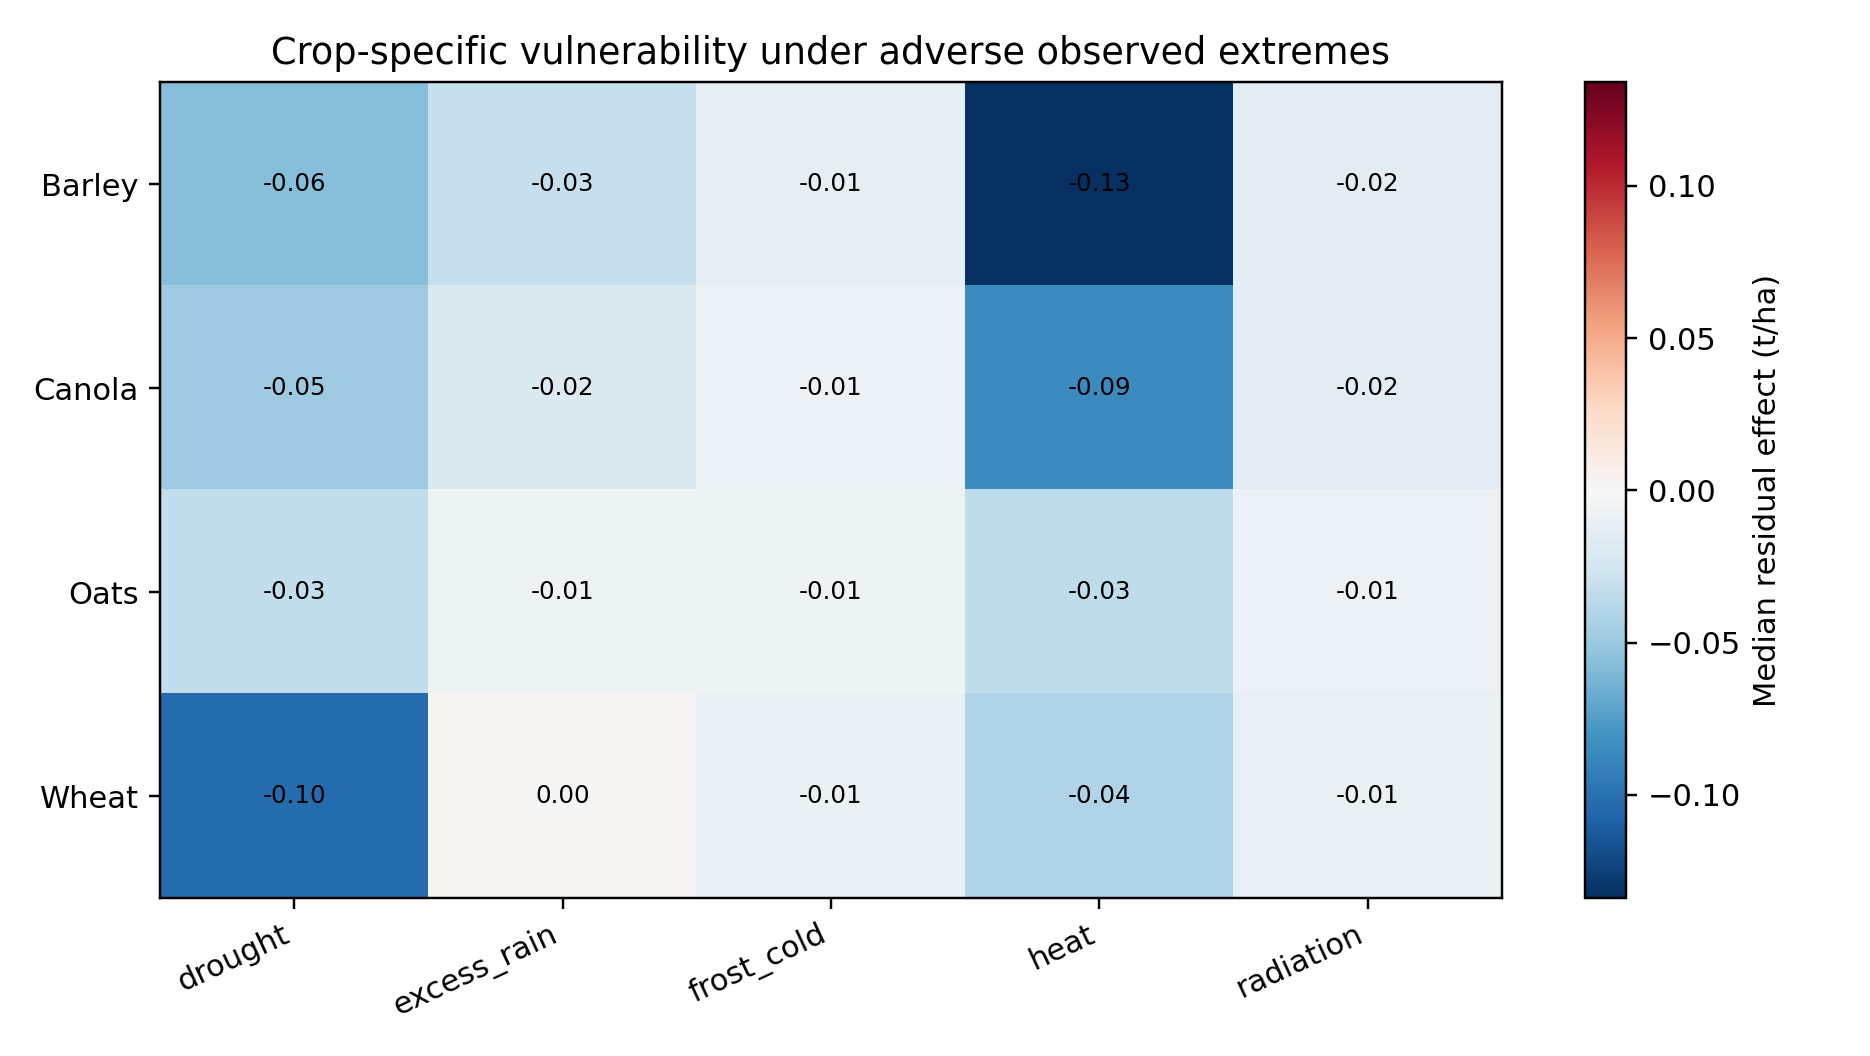
\includegraphics[width=0.86\linewidth]{fig07_crop_driver_vulnerability.png}
  \caption{Crop-specific vulnerability profiles under adverse observed driver-group extremes.}
  \label{fig:vulnerability}
\end{figure}

\begin{figure}[H]
  \centering
  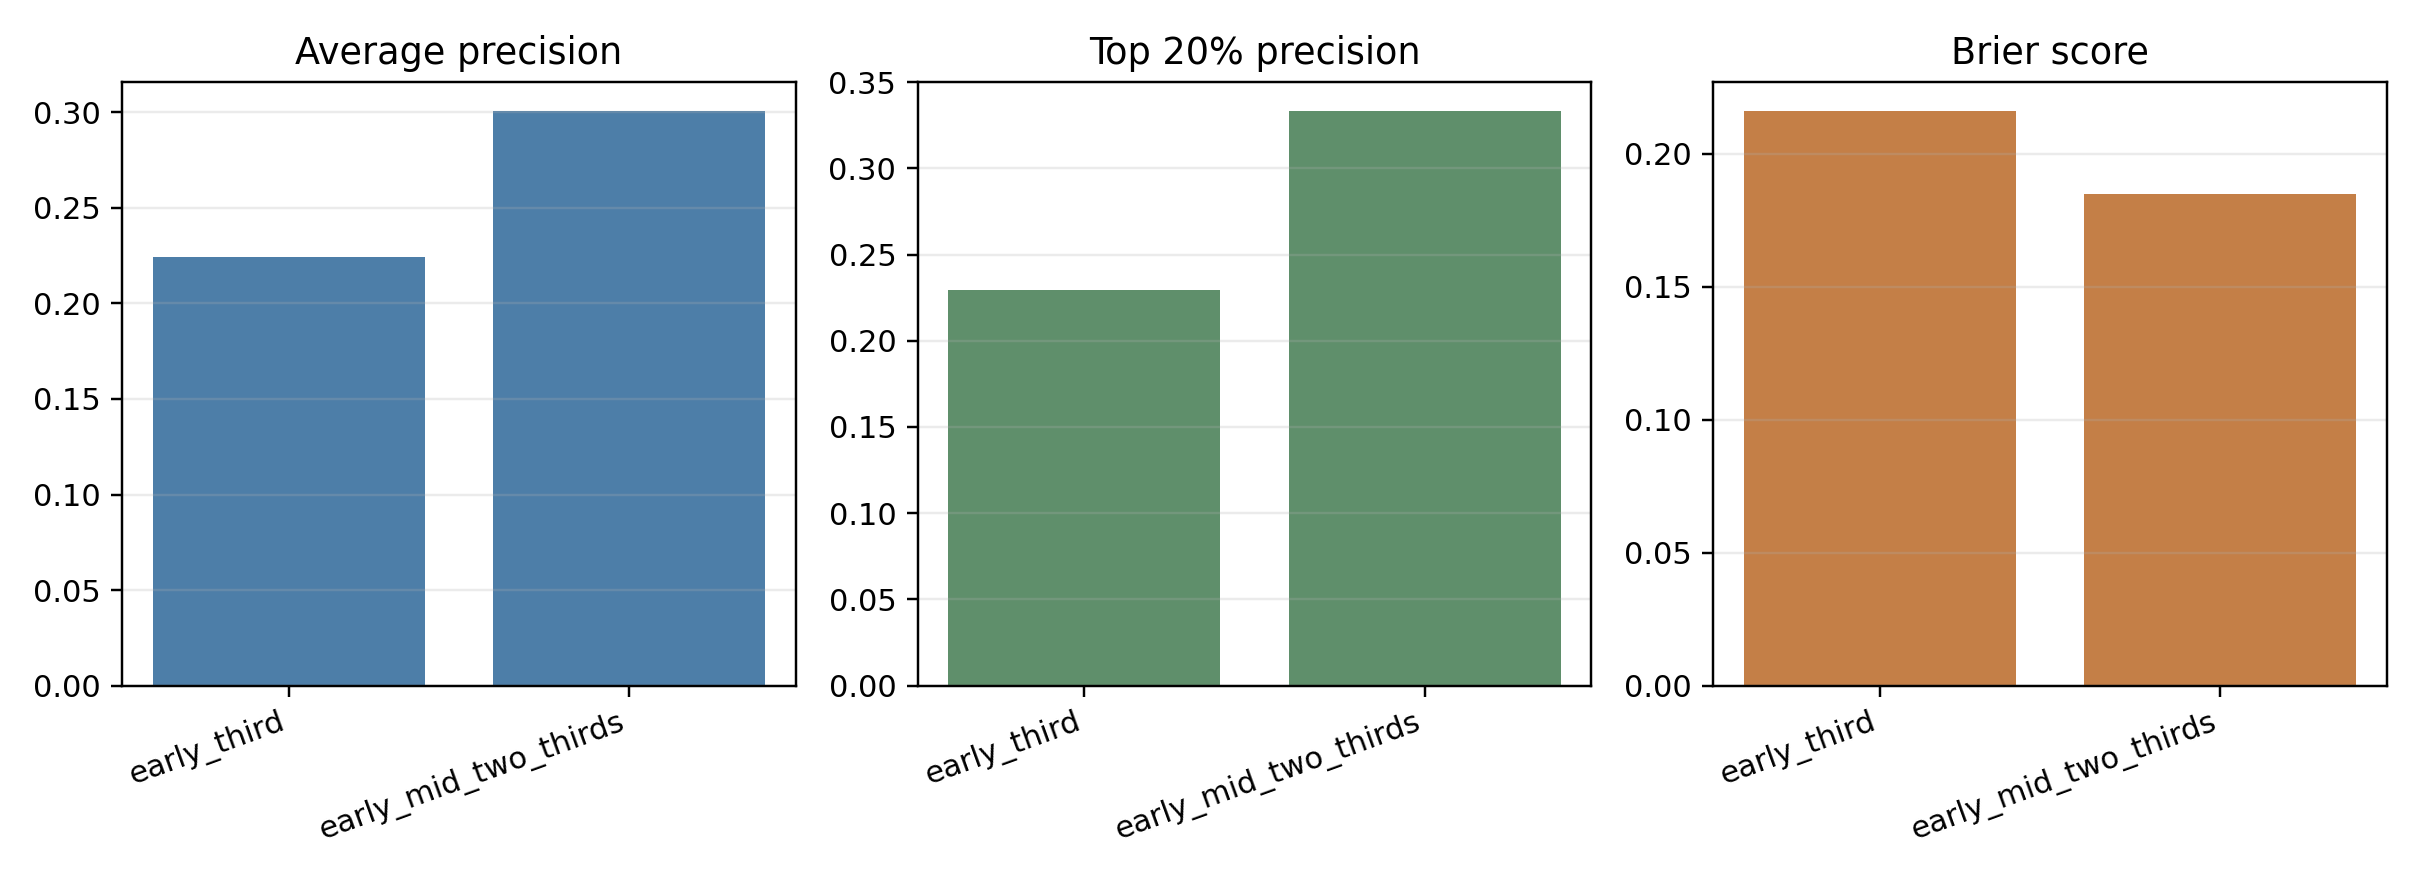
\includegraphics[width=\linewidth]{fig09_early_warning.png}
  \caption{Early-warning extension comparing early-season and early-plus-mid-season anomaly risk models.}
  \label{fig:warning}
\end{figure}

\section{Discussion}
The results show that the best research framing is not average yield prediction, but
event-level attribution of detrended low-yield anomalies. Grouped-SCAA improves over
the raw-yield baseline by aligning the model target with the anomaly definition and by
reporting physically interpretable driver groups. Observed analogs provide an important
plausibility check because they use weather seasons that actually occurred.

There are several limitations. The counterfactuals are model-internal predictive
associations; they are not causal effects in the sense of formal climate-event
attribution \citep{Hannart2016,Oldenborgh2021}. State-level aggregation hides
within-state variation in irrigation, soil, cultivar, and management. Linear detrending
is transparent, but alternative detrending choices may change anomaly membership
\citep{Meng2024}. Finally, the early-warning extension uses realized early-season
weather, not operational seasonal forecasts.

\section{Conclusion}
SCAA detects detrended low-yield anomalies and attributes them to sparse, physically
grouped weather counterfactuals. On U.S. Barley, Canola, Oats, and Wheat across
1990--2025, grouped-SCAA identifies crop-state-year claims such as heat exposure in
Canola or drought/dry-spell stress in Wheat, with explicit recovered t ha$^{-1}$ and
recoverable fractions. This provides a paper-ready contribution between crop-yield
prediction, interpretable machine learning, and cautious event-level weather
attribution.

\bibliographystyle{plainnat}
\bibliography{references}

\end{document}
